\documentclass[a4paper,12pt]{jarticle}

% レイアウト
\setlength{\hoffset}{0cm}
\setlength{\oddsidemargin}{-3mm}
\setlength{\evensidemargin}{-3cm}
\setlength{\marginparsep}{0cm}
\setlength{\marginparwidth}{0cm}
\setlength{\textheight}{24.7cm}
\setlength{\textwidth}{17cm}
\setlength{\topmargin}{-45pt}


\renewcommand{\baselinestretch}{1.3}
\renewcommand{\floatpagefraction}{1}
\renewcommand{\topfraction}{1}
\renewcommand{\bottomfraction}{1}
\renewcommand{\textfraction}{0}
\renewcommand\thefootnote{\arabic{footnote})}

% パッケージ
\usepackage[dvipdfmx]{graphicx}
\usepackage{amsmath,amssymb,epsfig}
\usepackage{eucal}
\usepackage{bm}
\usepackage{ascmac}
\usepackage{pifont}
\usepackage{multirow}
\usepackage{enumerate}
\usepackage{cases}
\usepackage{type1cm}
\usepackage{cancel}
\usepackage{url}
\usepackage{cite}
%\usepackage{color}
\usepackage[dvipdfmx]{color}
\usepackage{caption}
\usepackage[caption=false]{subfig}
\captionsetup[figure]{labelsep=space}

% 擬似コード作成用
\usepackage[ruled,vlined]{algorithm2e}
\usepackage{setspace}
\DeclareRelationFont{JY1}{mc}{it}{}{OT1}{cmr}{it}{}
\DeclareRelationFont{JT1}{mc}{it}{}{OT1}{cmr}{it}{}
\DeclareFontShape{JY1}{mc}{m}{it}{<5> <6> <7> <8> <9> <10> sgen*min
    <10.95><12><14.4><17.28><20.74><24.88> min10
    <-> min10}{}
\DeclareFontShape{JT1}{mc}{m}{it}{<5> <6> <7> <8> <9> <10> sgen*tmin
    <10.95><12><14.4><17.28><20.74><24.88> tmin10
    <-> tmin10}{}
\DeclareRelationFont{JY1}{mc}{sl}{}{OT1}{cmr}{sl}{}
\DeclareRelationFont{JT1}{mc}{sl}{}{OT1}{cmr}{sl}{}
\DeclareFontShape{JY1}{mc}{m}{sl}{<5> <6> <7> <8> <9> <10> sgen*min
    <10.95><12><14.4><17.28><20.74><24.88> min10
    <-> min10}{}
\DeclareFontShape{JT1}{mc}{m}{sl}{<5> <6> <7> <8> <9> <10> sgen*tmin
    <10.95><12><14.4><17.28><20.74><24.88> tmin10
    <-> tmin10}{}
\DeclareRelationFont{JY1}{mc}{sc}{}{OT1}{cmr}{sc}{}
\DeclareRelationFont{JT1}{mc}{sc}{}{OT1}{cmr}{sc}{}
\DeclareFontShape{JY1}{mc}{m}{sc}{<5> <6> <7> <8> <9> <10> sgen*min
    <10.95><12><14.4><17.28><20.74><24.88> min10
    <-> min10}{}
\DeclareFontShape{JT1}{mc}{m}{sc}{<5> <6> <7> <8> <9> <10> sgen*tmin
    <10.95><12><14.4><17.28><20.74><24.88> tmin10
    <-> tmin10}{}
\DeclareRelationFont{JY1}{gt}{it}{}{OT1}{cmbx}{it}{}
\DeclareRelationFont{JT1}{gt}{it}{}{OT1}{cmbx}{it}{}
\DeclareFontShape{JY1}{mc}{bx}{it}{<5> <6> <7> <8> <9> <10> sgen*goth
    <10.95><12><14.4><17.28><20.74><24.88> goth10
    <-> goth10}{}
\DeclareFontShape{JT1}{mc}{bx}{it}{<5> <6> <7> <8> <9> <10> sgen*tgoth
    <10.95><12><14.4><17.28><20.74><24.88> tgoth10
    <-> tgoth10}{}
\DeclareRelationFont{JY1}{gt}{sl}{}{OT1}{cmbx}{sl}{}
\DeclareRelationFont{JT1}{gt}{sl}{}{OT1}{cmbx}{sl}{}
\DeclareFontShape{JY1}{mc}{bx}{sl}{<5> <6> <7> <8> <9> <10> sgen*goth
    <10.95><12><14.4><17.28><20.74><24.88> goth10
    <-> goth10}{}
\DeclareFontShape{JT1}{mc}{bx}{sl}{<5> <6> <7> <8> <9> <10> sgen*tgoth
    <10.95><12><14.4><17.28><20.74><24.88> tgoth10
    <-> tgoth10}{}
\DeclareRelationFont{JY1}{gt}{sc}{}{OT1}{cmbx}{sc}{}
\DeclareRelationFont{JT1}{gt}{sc}{}{OT1}{cmbx}{sc}{}
\DeclareFontShape{JY1}{mc}{bx}{sc}{<5> <6> <7> <8> <9> <10> sgen*goth
    <10.95><12><14.4><17.28><20.74><24.88> goth10
    <-> goth10}{}
\DeclareFontShape{JT1}{mc}{bx}{sc}{<5> <6> <7> <8> <9> <10> sgen*tgoth
    <10.95><12><14.4><17.28><20.74><24.88> tgoth10
    <-> tgoth10}{}
\DeclareRelationFont{JY1}{gt}{it}{}{OT1}{cmr}{it}{}
\DeclareRelationFont{JT1}{gt}{it}{}{OT1}{cmr}{it}{}
\DeclareFontShape{JY1}{gt}{m}{it}{<5> <6> <7> <8> <9> <10> sgen*goth
    <10.95><12><14.4><17.28><20.74><24.88> goth10
    <-> goth10}{}
\DeclareFontShape{JT1}{gt}{m}{it}{<5> <6> <7> <8> <9> <10> sgen*tgoth
    <10.95><12><14.4><17.28><20.74><24.88> tgoth10
    <-> tgoth10}{}
\endinput
%%%% end of jdummy.def

% カウンタの設定
\setcounter{section}{0}
\setcounter{subsection}{0}
\setcounter{subsubsection}{0}
\setcounter{equation}{0}

% キャプションの図をFigに変更
\renewcommand{\figurename}{Fig.}
\renewcommand{\tablename}{Tab.}

% 式番号を式(章番号.番号)に
\makeatletter
\renewcommand{\theequation}{\arabic{section}.\arabic{equation}}
\@addtoreset{equation}{section}
\makeatother

% 表紙
\title{卒業論文\\
タイトル\\
% {\large No title}
}
\author{\vspace{90mm}\\
指導教員:\ 西田 \hspace{0mm} 健 准教授\\
九州工業大学\ \hspace{0mm} 工学部\\
機械知能工学科\ \hspace{0mm} 知能制御工学コース \\
\vspace{0mm}\\
学籍番号:\ xxxxxxxx\\
提出者氏名:\ 性 \hspace{0mm} 名\\\vspace{5mm}\\ }
\date{平成xx年\ x月\ xx日}

% ドキュメントの開始
\begin{document}
% 表紙
\titlepage
\maketitle
\thispagestyle{empty}
\newpage

% 概要
\begin{abstract}
% 垂直多関節ロボットを対象とした軌道計画について,多くの研究がなされている.
% 本研究では6軸の垂直多関節ロボットを対象とし,初期姿勢と目標姿勢を与えることでロボットが動作環境中の障害物を避けながら目標姿勢に到達するための経路生成手法を提案する.
% 具体的にはポテンシャル法とRRTアルゴリズムを組み合わせて構成した修正Transition-based RRT(T-RRT)の有効性を示す.
\end{abstract}
\thispagestyle{empty}

% 目次
\thispagestyle{empty}
\tableofcontents
\newpage

% 最初のやつ
\section{背景・目的}
\label{sec:背景・目的}
産業分野においてロボットの需要は高まってきている. しかし, これらのロボットの設置には様々な問題が伴う. 設置、ティーチング、利用に至るまでに少なからず知識と専門的な技術を要する. 今回の研究では, ロボットの導入部分にあたる動作環境構築に焦点を当てて問題解決の第一歩となるシステムの開発研究を行った. 


\section{原理}
\label{sec:原理}
\subsection{ROS}
\label{sec:ROS}

T-RRTの処理をAlgorithm~\ref{T-RRT}に示す.
%
\begin{algorithm}[b]
\caption{T-RRT Algorithm\label{T-RRT}}
\nl Define the configuration space (C-space) : $\mathcal{C}$\;
\nl Input the start $\bm{q}_{start}$ and the goal $\bm{q}_{goal}$\;
\nl \textcolor{red}{Define the cost function : Cost($\bm{q}$)}\;
\nl $\tau$.init($\bm{q}_{start}$)\;
\nl\While{GoalReached $=$ False \bf{and}\\\hspace{11mm} $iterations < \mathrm{MAX}$ $\mathrm{ITERATIONS}$ }{
 \nl $\bm{q}_{rand}$ $\longleftarrow$ randSample($\mathcal{C}$)\;
 \nl$\bm{q}_{near}$ $\longleftarrow$ NearestNode($\bm{q}_{sample}$,\ $\mathcal{C}$)\;
 \nl$\bm{q}_{new}$ $\longleftarrow$ GenNewNode($\bm{q}_{near}$,\ $\bm{q}_{sample}$)\;
 \nl\If{ $\bm{q}_{new} \neq \mathrm{NULL}$ \bf{and}\\\hspace{5mm}
         \textcolor{red}{$\mathrm{TransitionTest(}\bm{q}_{new},\ \bm{q}_{near}\mathrm{)} = True$} \bf{and}\\\hspace{5mm}
         \textcolor{red}{$\mathrm{MinExpandControl(}\bm{a},\ \bm{q}_{near},\ \bm{q}_{rand}\mathrm{)} = True$}
        }{
   \nl$\tau$ $\longleftarrow$ AddNode($\tau$,\ $\bm{q}_{new}$)\;
   \nl$\tau$ $\longleftarrow$ AddEdge($\tau$,\ $\bm{q}_{near}$,\ $\bm{q}_{new}$)\;
   \nl\If{ $\mathrm{CheckGoal(}\bm{q}_{new}\mathrm{)} = True$ }{
     \nl$GoalReached \longleftarrow True$\;
   }
 }
}
\end{algorithm}

% まず1行目で探索木$\tau$を初期化するために,開始位置$\bm{x}^{s}$,目標位置
% $\bm{x}^{g}$および探索エリアを初期条件として与える.
% 2行目では,探索開始前に評価関数としてCostFn($\bm{x}$)を与える.
% 3行目から探索ループに入り,4行目では,探索エリア内で障害物に含まれないラ
% ンダムな点$\bm{x}^{sample}$を設定する.

% 5行目では,探索木$\tau$の中で$\bm{x}^{sample}$に最も近い点
% $\bm{x}^{near}$を探索する.
% また,$\bm{x}^{near}$から$\bm{x}^{sample}$に対して距離を$\varepsilon$だ
% け伸ばした点を$\bm{x}^{new}$とする.
% ただし$|\bm{x}^{sample}-\bm{x}^{near}|<\varepsilon$となる場合には,
% $\bm{x}^{sample}$を$\bm{x}^{new}$とする.
% %
% 6行目では,$\bm{x}^{near}$から$\bm{x}^{new}$までの線分が障害物と干渉してい
% なければ$\bm{x}^{new}$として探索木$\tau$に登録し,$\bm{x}^{near}$と
% $\bm{x}^{new}$の接続情報を保存する.
% 干渉していれば,$\bm{x}^{new}$を破棄する.
% %
% 7行目では,TransitionTest関数により,新たなノード$\bm{x}^{new}$の登録の
% 判定を行う.
% %
% 10行目では,ゴール座標に到達しているかを確認する.
% CheckGoal関数は,$\bm{x}^{new}$と目標位置$\bm{x}^{g}$の偏差がしきい値
% を下回れば$True$を返す関数である.
% $True$が返された場合には,$\bm{x}^{new}$と$\bm{x}^{g}$を差分の長さで完
% 全に接続し処理を終了する.

% 以上の処理手順がRRTと異なるのは2行目と7行目である.
% 2行目のCostFn($\bm{x}$)の詳細は後述する.

% 7行目のTransitionTest関数の詳細をAlgorithm~\ref{transitionTest}に示す.
%
\begin{algorithm}[t]
\caption{TransitionTest($\bm{x}^{child}$,\ $\bm{x}^{parent}$)\label{transitionTest}}
 \nl$ChildCost \longleftarrow \rm{Cost(}$$\bm{x}^{child}$$\rm{)}$\;
 \nl$ParentCost \longleftarrow \rm{Cost(}$$\bm{x}^{parent}$$\rm{)}$\;

 \nl\If{$ChildCost \leq ParentCost$}{
   \nl\bf{return} $True$\;
 }

 % // コストの差と距離を計算
 \nl$\Delta C \longleftarrow \displaystyle\frac{ChildCost - ParentCost}{distance}$\;

 % // 確率計算
 \nl$TransitionProbability \longleftarrow \exp\left(-\displaystyle\frac{\Delta C}{K\cdot T}\right)$\;


 % // Check if we can accept it
 \nl\If{$Rand(0,\ 1) \leq TransitionProbability$}{
   \nl$T \longleftarrow T/\alpha$\;
   \nl$Failed \longleftarrow 0$\;
   \nl\bf{return} $True$\;
 } \nl\Else {
   \nl\If {$Failed \geq Failed_{max}$} {
     \nl$T \longleftarrow T\cdot\alpha$\;
     \nl$Failed \longleftarrow 0$\;
   } \nl\Else {
     \nl$Failed \longleftarrow Failed+1$\;
   }
   \nl\bf{return} $False$\;
 }
\end{algorithm}
%
この関数では,1行目と2行目で親ノード$\bm{x}^{parent}$,子ノード
$\bm{x}^{child}$に関する評価を算出する.
%
3行目でそれらの評価値を比較し,$ChildCost > ParentCost$の場合は,
\begin{equation}
\label{eq:cb}
  \Delta C = \frac{ChildCost - ParentCost}{distance}
\end{equation}
を算出する.
%
親ノードと子ノードの評価値の差と,ノード間距離に応じて定まる$\Delta C$を
用いて,それらのノードの組み合わせの採択を次式の確率関数$p$によって判定する.
\begin{equation}
\label{eq:ca}
  p = \begin{cases}
    \exp\left(-\displaystyle\frac{\Delta C}{K\cdot T}\right) &
       \mathrm{if}\ \  \Delta C >0 \\
    1.0 & \mathrm{otherwise}
  \end{cases}
\end{equation}
この関数の概形をFig.~\ref{fig:確率関数$p$}に示す.
ここで$K>0$は確率$p$の調整用の定数であり,開始位置と目標位置の評価値の平
均値で与える.
%
\begin{figure}[b]
  \centering
  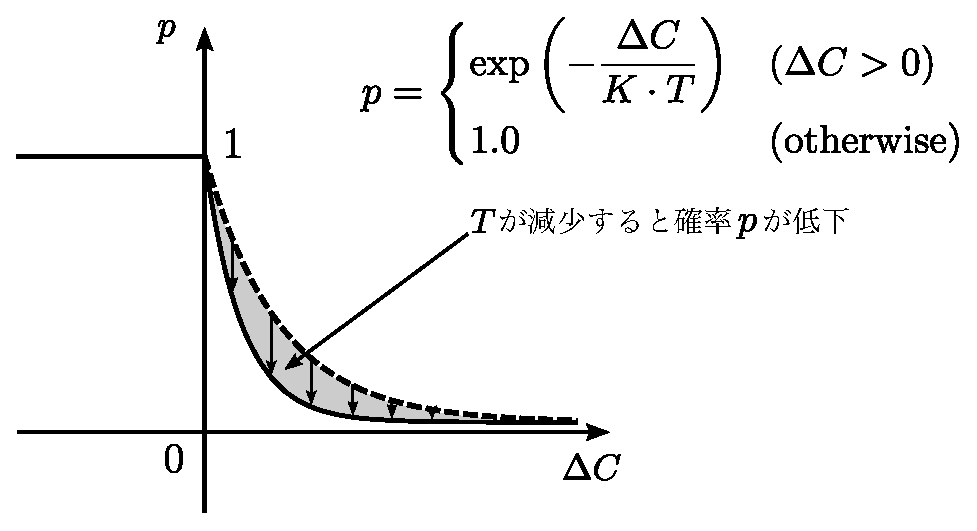
\includegraphics[clip,width=7cm]{../figure/eps/T-RRT_P.eps}
  \caption{The effect of $T$ on the probability function $p$.}
  \label{fig:確率関数$p$}
\end{figure}
%
$T$はTransitionTest関数の実行の度に調整される変数であり,確率$p$をループ
ごとに遷移させる役割を持つ.

%
$ChildCost > ParentCost$の場合,確率$p\ (\Delta C >0)$を利用し判定を行うフェーズ
に入る(Algorithm~\ref{transitionTest},10行目).
%
確率の範囲内であれば,注目する二つのノード間の経路が採択される.
%
このとき同時に,$T$を$\alpha\ (\alpha>0)$で除することで$T$の値を減少させる.
%
この操作により,次回のループでTransitionTest関数が実行され同じフェーズに
入った場合に,確率$p$の値が低くなるので,注目する二つのノード間の経路が
採択される確率が低くなる.
%
二つのノード間の経路が採択されない場合が一定回数以上続いた場合,すなわち
Algorithm~\ref{transitionTest}の変数$Failed$によるカウントがある一定
値以上に増加した場合には,変数$Failed$を初期化し,$T$を$\alpha$との乗算
によって値を再び増加させる.
% subsection T-RRT (end)

\subsection{Gazebo}
\label{sec:Gazebo}
なんでこのアルゴリズムを研究するのか?
% subsection 問題点 (end)

\subsection{RViz}
\label{sec:RViz}
ここがコアな部分だよ.
% subsection ポテンシャル関数を導入 (end)

\subsection{Point Cloud Library(PCL)}
\label{sec:Point Cloud Library(PCL)}
ポテンシャル関数もC-Spaceだと一工夫必要ですよ.を書く.
% subsection コンフィギュレーション空間での取り扱い (end)

% section モーションプランニング (end)

\subsection{ICPアルゴリズム}
\label{sec:ICPアルゴリズム}

\section{手法}
\label{sec:手法}
\subsection{仮想空間内での点群処理}
\label{sec:仮想空間内での点群処理}
ROSを使うよ.研究室で構築しているシステムの外観を説明するよ.
ROSを使えば実機でもシミュレーション上でもソフトウェアの部分で差異がない環境を実現できるよ.
% subsection 産業用ロボットのROS対応 (end)

\subsection{実物体とのマッチング}
\label{sec:実物体とのマッチング}
検証の段階で,実機を使わなくてもシミュレーションですべて確認できるよ.
% subsection 物理シミュレータの使用 (end)

\subsection{評価方法}
\label{sec:モーションプランニングについて}
MoveIt!(要説明)に準拠することで,リッチなGUIを使用しながらアルゴリズムの開発ができますよ.また世界中で提案されているアルゴリズムとの比較が容易ですよ.
またモーションプランニング部分はこの部分に着目して研究できるように産業用ロボットの物理シミュレータを用意し,有効性を確認できるようにしているよ.
% subsection モーションプランニングについて (end)

% section システム構成 (end)

\section{実験装置・環境}
\label{sec:実験装置・環境}


\section{実機での検証}
\label{sec:実機での検証}
\subsection{検証条件}
\label{sec:検証条件}
こんな条件で提案手法のアルゴリズムの有効性を確認します.
% subsection シミュレーション条件 (end)

\subsection{実験結果と考察}
\label{sec:実験結果と考察}
結果ドーン
% subsection 各種アルゴリズムと提案アルゴリズムの比較 (end)

% section シミュレーション (end)

\section{まとめ}
\label{sec:まとめ}
まとめ.どうなるかな???
% section まとめ (end)

% 謝辞
\section*{謝辞}
本論文作成にあたり御指導下さった九州工業大学大学院工学研究院機械知能工学研究系知能制御工学部門西田准教授に深く感謝致します.
さらに,日頃より御協力頂いた機械知能工学科制御工学教室の教職員の皆様ならびに,同教室西田研究室の皆様に感謝致します.

\section*{感想}
% 私たちはこの1年間この研究を望んで多くのこと
% を体験し,学びました.最初軽い気持ちでこの議題を
% 選んだのですが,つくづく後悔したものです.
% まぁ,なんだかんだ言いながら,
% こうしてつたない形ですが,
% 完成できてほっとしております.最初は先生にいろい
% ろ教えてもらいながら,大丈夫かなぁ?といぶかしみ
% ながら,少しずつしか進めることができなかったので
% すが,コツというのが,わかってきたのか,最後の方
% は一気にできてしまった気もします.ですが,きっと
% 最初からこつこつやってきたのがやっと自分たちの身
% についてきた結果だと思います.

\begin{thebibliography}{99}
\addcontentsline{toc}{section}{参考文献}
  \bibitem{Muhammad} Muhammad Zeeshan Malik; Amre Eizad; Muhammd Umer Khan, Path Planning Algorithms for mobile robots A Comprehensive Comparative Analysis, LAP LAMBERT Academic Publishing, 2014.
\end{thebibliography}

% 付録の始まり
\appendix
\def\thesection{付録\Alph{section}}
\def\thesubsection{\Alph{section}\arabic{subsection}}

\makeatletter
\renewcommand{\theequation}{\Alph{section}.\arabic{equation}}
\@addtoreset{equation}{section}
\makeatother
% \setcounter{page}{1}
% ODEの説明
\section{ }
\label{sec:}


% % 図の挿入

% \begin{figure}[b]
%  \begin{center}
%   \includegraphics[scale=0.9]{../figure/circuit.eps}
%   \caption{Uncontrolled converter}
%   \label{circuit}
%  \end{center}
% \end{figure}


% % 表の挿入

% \begin{table}[htb]
%   \begin{center}
%     \caption{各素子のパラメータ}
%     \begin{tabular}{c|c|c} \hline
%       定数名[単位] & 記号 & 値 \\ \hline \hline
%       周波数[Hz] & $f_U,f_V,f_W$ & 120 \\ \hline
%                      & $\phi_U$ & $\frac{2\pi}{3}$ \\
%       初期位相角[rad] & $\phi_V$ & $\frac{4\pi}{3}$ \\
%                      & $\phi_W$ & $2\pi$ \\ \hline
%       抵抗[$\Omega$] & $R$ & 10 \\ \hline
%     \end{tabular}
%     \label{param}
%   \end{center}
% \end{table}


% % 図の挿入

% \begin{figure}[tb]
%  \centering
%  \vspace{0.5cm}
%  \includegraphics[scale=0.85]{../figure/waves.eps}\\
%  \hspace{0.0cm}
%  % 入力と出力\\
%  % \\
%  % \vspace{1.2cm}
%  % \includegraphics[scale=0.825]{../figure/output.eps}\\
%  % (b) 出力の電位\\
%  % \\
%  \caption{シミュレーションにより得られた各電源電圧(上)と出力電位(下)の波形}
%  \label{wave}
% \end{figure}

% \newpage

% % 図を並べて挿入

% \begin{figure}[tb]
%  \centering
%  \subfloat[区間1における回路動作]{\includegraphics[scale=0.5]{../figure/kukan_1.eps}}
%  \hspace{1.5cm}
%  \subfloat[区間2における回路動作]{\includegraphics[scale=0.5]{../figure/kukan_2.eps}}
% \\
%  \vspace{0.5cm}
%  \subfloat[区間3における回路動作]{\includegraphics[scale=0.5]{../figure/kukan_3.eps}}
%  \hspace{1.5cm}
%  \subfloat[区間4における回路動作]{\includegraphics[scale=0.5]{../figure/kukan_4.eps}}
% \\
%  \vspace{0.5cm}
%  \subfloat[区間5における回路動作]{\includegraphics[scale=0.5]{../figure/kukan_5.eps}}
%  \hspace{1.5cm}
%  \subfloat[区間6における回路動作]{\includegraphics[scale=0.5]{../figure/kukan_6.eps}}
% \\
%  \caption{各区間での回路動作の様子}
%  \label{circuit_kaku}
% \end{figure}

% % 文中へのラベリング
% {\bf Fig. }\ref{circuit_kaku}に示す〜

% % 参考文献
% \begin{thebibliography}{99}
% \addcontentsline{toc}{section}{参考文献}
% \bibitem{1} T.Sakamoto,”Lecture Note of Advanced Electrical Drive Control System”,pp.19-20.
% \bibitem{2} 坪島 茂彦,”誘導電動機 -基礎から制御まで-”,東京電機大学出版局,pp.13-17,2006.
% \end{thebibliography}

\end{document}
